% https://github.com/python/cpython/blob/3.9/Lib/colorsys.py
% https://github.com/python/cpython/blob/3.12/Lib/colorsys.py
% https://github.com/python/cpython/blob/3.14/Lib/colorsys.py
% https://gist.github.com/yoggy/8999625
% https://www.cnblogs.com/Imageshop/archive/2013/02/02/2889897.html
% https://www.toolkk.com/tools/rgb-cielab-converter
% https://www.cnblogs.com/hrlnw/p/4126017.html

\documentclass{article}

\usepackage{bm}
\usepackage{ctex}
\usepackage{float}
\usepackage{xcolor}
\usepackage{datetime}
\usepackage{geometry}
\usepackage{graphicx}
\usepackage{enumitem}
\usepackage{amsmath, amssymb, amsfonts, mathrsfs}
\usepackage[fontsize = 12pt]{fontsize}

\newcommand{\diff}[2]{\dfrac{\mathrm{d}#1}{\mathrm{d}#2}}
\newcommand{\diffn}[3]{\dfrac{\mathrm{d}^{#3}#1}{\mathrm{d}#2^{#3}}}
\newcommand{\eval}[2]{\left.#1\right|_{#2}}
\newcommand{\e}{\mathrm{e}}
\renewcommand{\d}{\mathrm{d}}
\newcommand{\mathsize}{\fontsize{8pt}{11pt}\selectfont}

\geometry{
    a4paper,
    left = 2.5cm,
    right = 2.5cm,
    top = 2cm,
    bottom = 2cm
}

\setitemize[1]{
    itemsep = 0pt,
    partopsep = 0pt,
    parsep = \parskip,
    topsep = 5pt
}

\title{图像处理：第四次作业}
\author{叶炳辉 \quad 202528017729004 \quad 人工智能学院}
\date{\currenttime,\ \today}



\begin{document}\maketitle

\section*{颜色空间及其各通道含义}

% RGB：适合用于显示设备，易于理解，但不适合直接进行颜色分析。
% HSV/HSL：更接近人眼对颜色的感知，适用于图像分割、目标追踪等应用。
% Lab：设备无关，适用于高精度颜色管理和色彩匹配。
% YCbCr：适用于视频压缩和编码，能有效减少数据量。

\paragraph*{1. RGB}~{}

Red Green Blue 红绿蓝色彩空间，这是一个加色法模型，基于人类眼睛视网膜对三种波长光的敏感特性，通道含义：

\begin{itemize}
    \item R：红色分量，通常取值在 $[0,\ 255]$ 范围；
    \item G：绿色分量，通常取值在 $[0,\ 255]$ 范围；
    \item B：蓝色分量，通常取值在 $[0,\ 255]$ 范围。
\end{itemize}

\begin{figure}[H]
    \centering
    \includegraphics*[scale=0.1,trim=350 450 350 250,clip]{./figs/RGB.jpeg}
    \caption{RGB}
\end{figure}

RGB 是最基本的颜色模型，面向如显示器、摄像头、扫描仪等硬件，三种颜色叠加越强，亮度越高，即 $(255,\ 255,\ 255)$ 代表纯白和 $(0,\ 0,\ 0)$ 代表纯黑，几何空间中表现为一个立方体。RGB 容易理解，但不合适直接进行颜色分析。

\paragraph*{2. NTSC}~{}

National Television System Committee 色域，这是一个用于电视机广播传输标准协议，目的是为了兼容黑白电视信号并节省传输带宽，通道含义：

\begin{itemize}
    \item Y：Luminance 亮度分量，如果只显示 Y 分量，就是黑白图像，包含了图像的细节和轮廓信息；
    \item I：In-phase 同相分量，代表从橙色到青色的色调变化，人类肉眼对该轴的颜色比较敏感；
    \item Q：Quadrature 正交分量，代表从紫色到黄绿色的色调变化，人类肉眼对该轴的颜色不敏感，因此带宽可以压缩得更低。
\end{itemize}
\begin{align*}
    \left[\begin{matrix}
        Y \\
        I \\
        Q \\
    \end{matrix}\right]&=\left[\begin{matrix}
        0.299 & 0.587 & 0.114 \\
        0.596 & -0.274 & -0.322 \\
        0.211 & -0.523 & 0.312 \\
    \end{matrix}\right]\left[\begin{matrix}
        R \\
        G \\
        B \\
    \end{matrix}\right]
    \\
    \left[\begin{matrix}
        R \\
        G \\
        B \\
    \end{matrix}\right]&=\left[\begin{matrix}
        1.000 & 0.956 & 0.621 \\
        1.000 & -0.272 & -0.647 \\
        1.000 & -1.106 & 1.703 \\
    \end{matrix}\right]\left[\begin{matrix}
        Y \\
        I \\
        Q \\
    \end{matrix}\right]
\end{align*}

NTSC 色彩空间被广泛运用于电视行业，Y 分量与 I、Q 分量分离，解决了彩色与黑白电视的兼容性问题。

\paragraph*{3. YCbCr}~{}

这是 RGB 的一种线性变换后的色彩空间，YCbCr 色域广泛应用于数字视频和图像压缩标准中，其通道含义：

\begin{itemize}
    \item Y：Luma 亮度分量，这里的 Y 是经过伽马校正后的亮度；
    \item Cb：Chroma Blue 蓝色色度分量，反映蓝色分量与亮度值的差异，即 B-Y；
    \item Cr：Chroma Red 红色色度分量，反映红色分量与亮度值的差异，即 R-Y。
\end{itemize}
\begin{align*}
    \left[\begin{matrix}
        Y \\
        Cb \\
        Cr \\
    \end{matrix}\right]=\left[\begin{matrix}
        16 \\
        128 \\
        128 \\
    \end{matrix}\right]+\left[\begin{matrix}
        65.481 & 128.553 & 24.966 \\
        -37.797 & -74.203 & 112.000 \\
        112.000 & -93.786 & -18.214 \\
    \end{matrix}\right]\cdot\dfrac{1}{256({\rm CS})\ /\ 255({\rm Math})}\cdot\left[\begin{matrix}
        R \\
        G \\
        B \\
    \end{matrix}\right]
\end{align*}
\begin{mathsize}\vspace*{-1.5em}
    \begin{align*}
        Y&=16+\{[(R<<6) + (R<<1) + (G<<7) + G + (B<<4) + (B<<3) + B]>>8\}
        \\
        Cb&=128+\{[-(R<<5)-(R<<2)-(R<<1)-(G<<6)-(G<<3)-(G<<1)+(B<<7)-(B<<4)]>>8\}
        \\
        Cr&=128+\{[(R<<7)-(R<<4)-(G<<6)-(G<<5)+(G<<1)-(B<<4)-(B<<1)]>>8\}
    \end{align*}
\end{mathsize}

YCbCr 色域应用很广，包括 JPEG 图片压缩、MPEG 视频压缩、DVD、数字电视等。因为人眼对亮度 Y 敏感，对色调 Cb、Cr 不敏感，在压缩时常保留 Y 的全分辨率，而对 Cb、Cr 进行降采样，从而大幅度减小数据量。

\begin{figure}[H]
	\centering
	\begin{minipage}{0.32\linewidth}
		\centering
		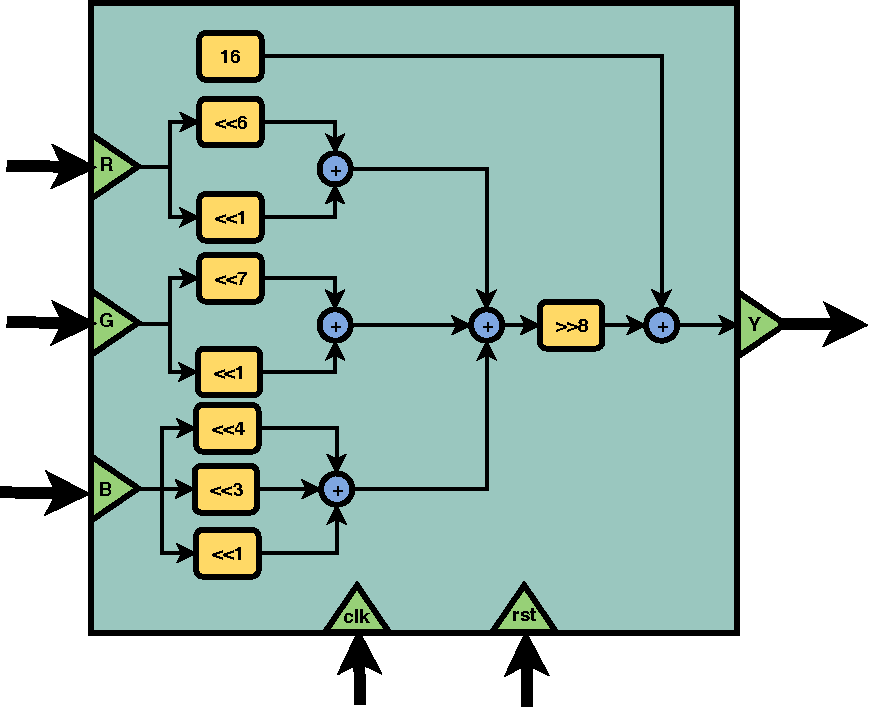
\includegraphics[width=1\linewidth]{./figs/RGB2Y.pdf}
		\caption{RGB $\to$ Y}
	\end{minipage}
	\begin{minipage}{0.32\linewidth}
		\centering
		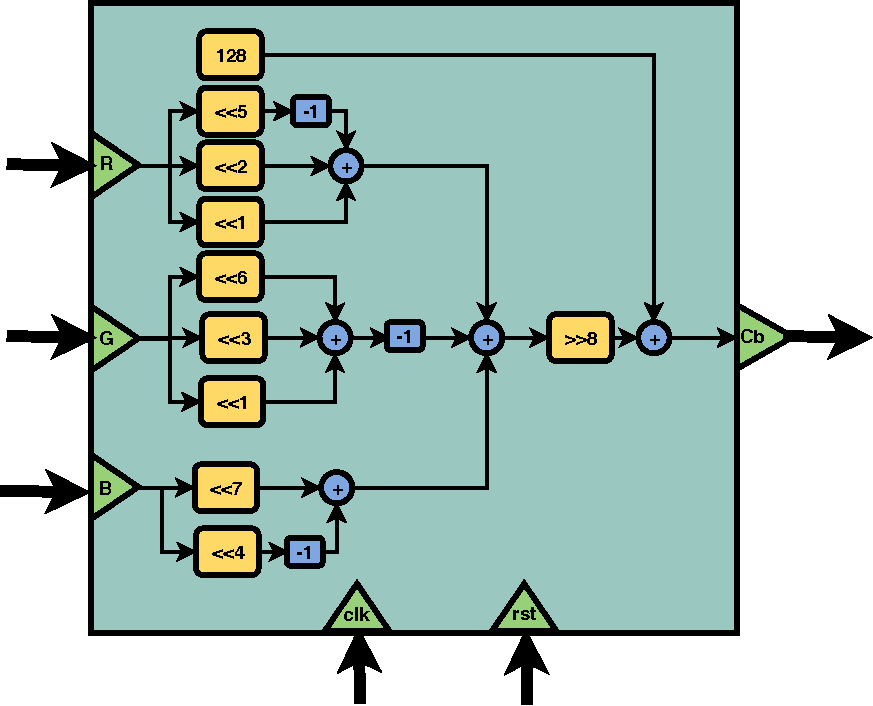
\includegraphics[width=1\linewidth]{./figs/RGB2Cb.pdf}
		\caption{RGB $\to$ Cb}
	\end{minipage}
    \begin{minipage}{0.32\linewidth}
		\centering
		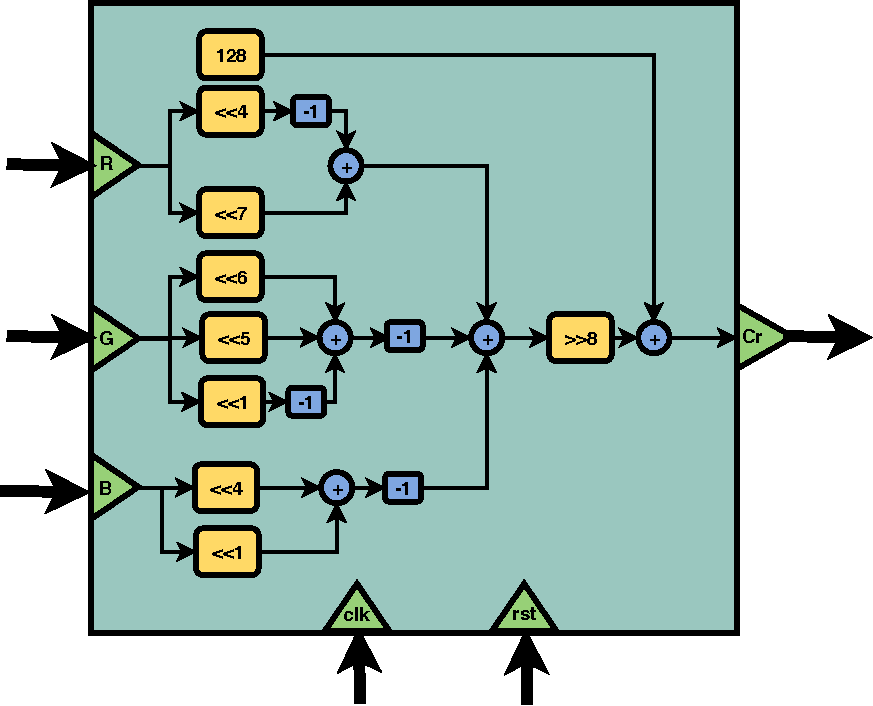
\includegraphics[width=1\linewidth]{./figs/RGB2Cr.pdf}
		\caption{RGB $\to$ Cr}
	\end{minipage}
\end{figure}

\paragraph*{4. HSV}~{}

Hue Saturation Value 色相饱和度明度色域空间，旨在模仿人类描述颜色的直观方式，而非机器混合光线的方式，通道含义：

\begin{itemize}
    \item H：色相，用角度度量（$0^{\circ}\sim360^{\circ}$），其中 $0^{\circ}$ 是红色，$120^{\circ}$ 是绿色，$240^{\circ}$ 是蓝色，$60^{\circ}$ 是黄色，$180^{\circ}$ 是青色，$300^{\circ}$ 洋红，它代表了颜色的种类；
    \item S：饱和度表示颜色的纯度或深浅，值越高颜色越鲜艳越纯，值为 0 时变为灰度；
    \item V：明度表示颜色的明亮程度，0\% 为最黑，100\% 为最亮，但需要注意的是，HSV 色域中，纯蓝和纯白都可以是 100\%，这与人类眼睛感知有偏差。
\end{itemize}
\begin{align*}
    R'=\dfrac{R}{255}\qquad G'&=\dfrac{G}{255}\qquad B'=\dfrac{B}{255}
    \\
    C_{\max}=\max\{R',\ G',\ B'\}&\qquad C_{\min}=\min\{R',\ G',\ B'\}
    \\
    \Delta=&C_{\max}-C_{\min}
\end{align*}
\vspace*{-2.5em}
\begin{align*}
    H&=\begin{cases}
        0^{\circ},\qquad \Delta=0
        \\[10pt]
        60^{\circ}\times\left(\dfrac{G'-B'}{\Delta}+0\right),\qquad C_{\max}=R'
        \\[10pt]
        60^{\circ}\times\left(\dfrac{B'-R'}{\Delta}+2\right),\qquad C_{\max}=G'
        \\[10pt]
        60^{\circ}\times\left(\dfrac{R'-G'}{\Delta}+4\right),\qquad C_{\max}=B'
    \end{cases}
    \\
    S&=\begin{cases}
        0,\qquad C_{\max}=0
        \\[10pt]
        \dfrac{\Delta}{C_{\max}},\qquad C_{\max}\neq0
    \end{cases}
    \\
    V&=C_{\max}
\end{align*}

HSV 色彩空间直观分离色相、饱和度和明度，符号人类对颜色的描述，对光照不敏感的时候，H 和 S 分量与 V 分量分离，适合颜色识别任务，几何空间通常呈现倒圆锥或六角锥体。

\paragraph*{5. CMY}~{}

Cyan Magenta Yellow 青洋黄色彩空间，这是一种减色法模型，基于颜料和油墨吸收光线的特性，通道含义：

\begin{itemize}
    \item C：青色油墨浓度，吸收红光，反射绿光和蓝光；
    \item M：洋红油墨浓度，吸收绿光，反射红光和蓝光；
    \item Y：黄色油墨浓度，吸收蓝光，反射红光和绿光。
\end{itemize}
\begin{align*}
    \left[\begin{matrix}
        C \\
        M \\
        Y \\
    \end{matrix}\right]=\left[\begin{matrix}
        255 \\
        255 \\
        255 \\
    \end{matrix}\right]-\left[\begin{matrix}
        R \\
        G \\
        B \\
    \end{matrix}\right]&\Longleftrightarrow\left[\begin{matrix}
        R \\
        G \\
        B \\
    \end{matrix}\right]=\left[\begin{matrix}
        255 \\
        255 \\
        255 \\
    \end{matrix}\right]-\left[\begin{matrix}
        C \\
        M \\
        Y \\
    \end{matrix}\right]
    \\
    K=\min&\{C,\ M,\ Y\}
\end{align*}

CMY 主要用于彩色打印和印刷，理论上 C + M + Y 为黑色，但实际上混合后是深褐色，因此工程应用中通常加上黑色形成 CMYK 模型，以获得纯正的黑色并节省彩色油墨。

\paragraph*{6. HSI}~{}

Hue Saturation Intensity 色相饱和度强度色域空间，这是一种与 HSV 类似的感知模型，但在亮度上定义了更符合光学解释的算法，其通道含义：

\begin{itemize}
    \item H：色相用角度度量（$0^{\circ}\sim360^{\circ}$），其中 $0^{\circ}$ 是红色，$120^{\circ}$ 是绿色，$240^{\circ}$ 是蓝色，$60^{\circ}$ 是黄色，$180^{\circ}$ 是青色，$300^{\circ}$ 洋红，它代表了颜色的种类；
    \item S：饱和度受强度 I 的影响，表示颜色被白光稀释的程度；
    \item I：强度直接定义为 RGB 三分量的算术平均值。
\end{itemize}
\begin{align*}
    \theta=\arccos&\left[\dfrac{\displaystyle(R-G)+(R-B)}{\displaystyle2\sqrt{(R-G)^2+(R-B)(G-B)}} \right]
    \\
    H=\begin{cases}
        \theta,\qquad B\leqslant G
        \\[10pt]
        360^{\circ}-\theta,\qquad B>G
    \end{cases}&\qquad S=1-\dfrac{3\min\{R,\ G,\ B\}}{R+G+B}\qquad I=\dfrac{R+G+B}{3}
\end{align*}
\vspace*{-1em}
\begin{align*}
    {\rm RG sector}(0^{\circ}\leqslant H<120^{\circ})&\implies\begin{cases}
        H=H-0^{\circ}
        \\[10pt]
        B=I(1-S)
        \\[10pt]
        R=I\left[1+\dfrac{S\cos H}{\cos(60^{\circ}-H)}\right]
        \\[10pt]
        G=3I-(B+R)
    \end{cases}
    \\
    {\rm GB sector}(120^{\circ}\leqslant H<240^{\circ})&\implies\begin{cases}
        H=H-120^{\circ}
        \\[10pt]
        R=I(1-S)
        \\[10pt]
        G=I\left[1+\dfrac{S\cos H}{\cos(60^{\circ}-H)}\right]
        \\[10pt]
        B=3I-(R+G)
    \end{cases}
    \\
    {\rm BR sector}(240^{\circ}\leqslant H<360^{\circ})&\implies\begin{cases}
        H=H-240^{\circ}
        \\[10pt]
        G=I(1-S)
        \\[10pt]
        B=I\left[1+\dfrac{S\cos H}{\cos(60^{\circ}-H)}\right]
        \\[10pt]
        R=3I-(G+B)
    \end{cases}
\end{align*}

HSI 解耦性好，强度 I 与图像的颜色信息完全无关，这使得它非常适合图像处理算法，譬如直方图均衡化，可以在不改变图像颜色的情况下仅处理亮度，常用于机器视觉和图像分析算法中。

\paragraph*{7. CIELab}~{\bfseries\textcolor{red}{补充}}

这是一个基于人类肉眼对颜色的感知，设备无关的颜色空间，旨在实现感知均匀性，通道含义：

\begin{itemize}
    \item L：亮度，取值 0 为纯黑，取值 100 为纯白，它模拟人类眼睛对亮度的非线性反应；
    \item a：红绿轴分量，正值代表红色，负值代表绿色；
    \item b：黄蓝轴分量，正值代表黄色，负值代表蓝色。
\end{itemize}
\begin{align*}
    \begin{cases}
        R=\gamma\left(\dfrac{r}{255}\right)
        \\[10pt]
        G=\gamma\left(\dfrac{g}{255}\right)
        \\[10pt]
        B=\gamma\left(\dfrac{b}{255}\right)
    \end{cases}\qquad\gamma(x)=\begin{cases}
            \left(\dfrac{x+0.055}{1.055}\right)^{2.4}\qquad x>0.04045
            \\[10pt]
            \dfrac{x}{12.92}\qquad\qquad\qquad\ x\leqslant0.04045
        \end{cases}
\end{align*}
\begin{align*}
    \left[\begin{matrix}
        X \\
        Y \\
        Z \\
    \end{matrix}\right]=\left[\begin{matrix}
        0.4124 & 0.3576 & 0.1805 \\
        0.2126 & 0.7152 & 0.0722 \\
        0.0193 & 0.1192 & 0.9505 \\
    \end{matrix}\right]\left[\begin{matrix}
        R \\
        G \\
        B \\
    \end{matrix}\right]
\end{align*}
\begin{align*}
    \begin{cases}
        L=116f\left(\dfrac{Y}{\mathbb{Y}}\right)-16
        \\[10pt]
        a=500\left[f\left(\dfrac{X}{\mathbb{X}}\right)-f\left(\dfrac{Y}{\mathbb{Y}}\right)\right]
        \\[10pt]
        b=200\left[f\left(\dfrac{Y}{\mathbb{Y}}\right)-f\left(\dfrac{Z}{\mathbb{Z}}\right)\right]
    \end{cases}\qquad \mathbb{X},\mathbb{Y},\mathbb{Z}=1
\end{align*}
\begin{align*}
    f(t)=\begin{cases}
        \displaystyle\sqrt[3]{t}\qquad\qquad\qquad\quad\ \ t>\left(\dfrac{6}{29}\right)^3
        \\
        \displaystyle\dfrac{1}{3}\left(\dfrac{29}{6}\right)^2t+\dfrac{4}{29}\qquad t\leqslant\left(\dfrac{6}{29}\right)^3
    \end{cases}
\end{align*}

其中 $\gamma(x)$ 函数是用来对图象进行非线性色调编辑的，目的是提高图像对比度，这个函数不唯一。CIELab 色域最宽，可以描述人眼可见的所有颜色，覆盖范围超过 RGB 和 CMYK 色彩空间，该色域空间中两点间的欧氏距离与人眼感知色差大致成正比，具有均匀性，因此广泛用于色彩管理系统、不同设备间颜色转换中介以及工业色差检测。



\end{document}